\section{Introduction}
\label{sec:intro}

%   Non-linear arithmetic over ℝ and δ-satisfiability
%       what it is
%           reasoning about continuous systems
%       Applications 
%           hybrid / embedded / cyber physical systems
%       how it is done
%           normal sat is undecidable
%           δ-sat leverage on finite precision arithmetic what can be efficiently performed by computer


%Software often interact with the physical world. Plant controllers, robots, cars, etc., all theses systems contains sensors and actuators. Validating such systems requires requires method to reason not only about the software part, but also the environment, usually described by continuous equations.

Verification problems of complex embedded software can be reduced to solving logic formulas that contain continous, typically nonlinear, real functions. The framework of delta-decision procedures~\cite{DBLP:conf/lics/GaoAC12,DBLP:conf/fmcad/GaoKC13} estabishes that, under reasonable relaxations, nonlinear SMT formulas over the reals are in principle as solvable as SAT problems. Indeed, using solvers for nonlinear theories as the algorithmic engines, straightforward bounded model checking has already shown promise on nonlinear hybrid systems~\cite{}. Naturally, for enhancing scability or going beyond bounded safety, more advanced verification techniques need to be introduced. 

Interpolants...\todo[inline]{a transition sentence saying why interpolants are important.} Given two formulas $A$ and $B$, such that $A ∧ B$ is unsatisfiable, an interpolant $I$ is a formula satisfying: (1) $A \vdash I$, (2) $B ∧ I \vdash ⊥$, and (3) $I$ contains only variables common to $A$ and $B$.
Craig interpolation can be seen as a weaker, less expensive replacement for quantifier elimination.
Therefore, it has found many applications in verifications:
as an heuristic to compute inductive invariant~\cite{DBLP:conf/cav/McMillan03,DBLP:conf/vmcai/McMillan07,DBLP:conf/sas/McMillan11},
for predicate discovery in abstraction refinement loops~\cite{DBLP:conf/cav/McMillan06},
inter procedural analysis~\cite{DBLP:conf/vmcai/AlbarghouthiGC12,DBLP:conf/cav/AlbarghouthiLGC12},
shape analysis~\cite{DBLP:conf/esop/AlbarghouthiBCK15},
fault-localisation~\cite{DBLP:conf/fm/ErmisSW12,DBLP:conf/vmcai/ChristESW13,DBLP:conf/sigsoft/SchafSW13}, etc.

In this paper, we present methods that transform proofs traces from delta-decision procedures into Craig interpolants for nonliner formulas over the reals. To do so, we extract interpolants from proofs of unsatisfiability generated by delta-decision procedures~\cite{DBLP:conf/synasc/GaoKC14} based on Interval Constraint Propagation (ICP)~\cite{}. 

A delta-decision problem relaxes the standard decision problem by allowing one-sided delta-bounded errors on the decisions. Instead of asking whether a formula has a satisfiable assignment or not, we ask if it is delta-satisfiable or unsatisfiable. Here, a formula is delta-satisfiable if it would be satisfiable under some {\em delta-perturbation}. On the other hand, when the algorithm determines that the formula is ``unsatisfiable," no numerical error can be involved. Indeed, we can extract proofs of unsatisfiability from such answers, even though the search algorithms involve numerical errors. This is accomplished by analyzing the execution trace of the search tree based on the ICP algorithm. 

The core ICP algorithm uses a {\em branch-and-prune} loop that zooms-in to boxes that contain delta-solutions for a system of constraints, or reports conflicts when no delta-solutions exists. The loop consists of two main steps:
\begin{itemize}
\item Use interval arithmetic to maintain overapproximations of the solution sets, so that one can ``prune" out the part of the state space that does not contain solutions.
\item When the pruning operation does not make progress, one can perform a depth-first search by ``branching" on variables and restart pruning operations on a subset of the domain. 
\end{itemize}
The loop is continued until either a small enough box that may contain a solution is found, or any conflict among the constraints is observed.

When a formula is unsatisfiable, the execution trace of the algorithm becomes can be seen as a proof tree that divides the space into small hypercubes and associating a constraint to each hypercube~\cite{DBLP:conf/synasc/GaoKC14}. Consequently, the interpolation algorithm can traverse this proof tree to construct the interpolant. To each leaf in the proof, we associate ⊤ or ⊥ depending on the source of the contradiction. The inner nodes of the proof tree correspond to case splits and are handled in a manner reminiscent of Pudl{\'a}k's algorithm~\cite{MR1472134}. Common variables are kept as branching points and $A$,$B$ local variables are eliminated. A simple example of the method is as follows:
\begin{example}
Let $A$ be $y≥x²$ and $B$ by $y ≤ -\cos(x) + 0.8$ over the domain $x∈[-1,1]$, $y∈[-1,1]$.
A δ-decision procedure uses $A$ and $B$ to contract the domains of $x$ and $y$ by removing the parts that be shown empty using interval arithmetic.
Figure~\ref{fig:example} shows a sequence of contraction proving the unsatisfiability of the formula.
As the contraction occurs, we color the region of the space by the color of the \emph{opposite} formula.
When the interval constraint propagation has finished all the initial domain is associated to either $A$ or $B$.
The interpolant $I$ is the parts corresponding to $A$.
$I$ is $y ≥ 0 ∧ (0.26 ≤ y ∨ (y ≤ 0.26 ∧ -0.51 ≤ x ≤ 0.51))$.

\begin{figure}
\centering
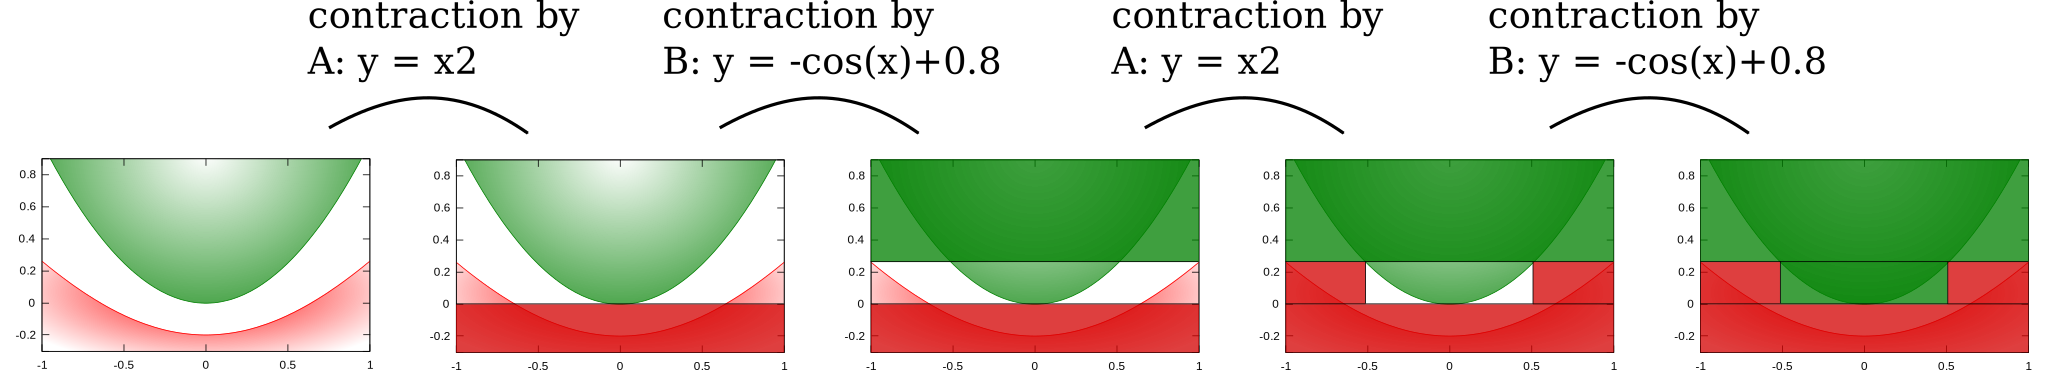
\includegraphics[scale=0.04]{img/example.pdf}
\caption{
    Interval constraint propagation and interpolant construction where $A$ is $y≥x²$ and $B$ is $y ≤ -\cos(x) + 0.8$ over the domain $x∈[-1,1]$, $y∈[-1,1]$.
    The $A$ is shown in green and $B$ in red.
    The final interpolant is the green part of the space.
}
\label{fig:example}
\end{figure}
\end{example}

We have implemented this on top of \dReal and we tested it with examples from geometric theorem proving, robotic design, and hybrid system verification.  

% Outline of the paper
In Section~\ref{sec:prelim}, we review notions related to interpolation, nonlinear arithmetic over the Reals and δ-decision procedures.
In Section~\ref{sec:itp}, we introduce our interpolation algorithm.
In Section~\ref{sec:eval}, we present and evaluate our implementation.
We review the related work and sketch future research direction in Section~\ref{sec:related}.
Finally, we conclude in Section~\ref{sec:concl}.

%Given two formulas which conjunction is unsatisfiable, the Craig interpolant~\cite{MR0104564} is a formula over the common variables that serves

%reasoning about the combined system of software and the physical environment. Modeling such environment typically requires extensive use of continuous functions over real numbers, such as solution functions of nonlinear differential equations. Thus solving logic formulas in nonlinear theories over the real numbers is a basic requirement for verification. 
%Unfortunately, automated reasoning for about nonlinear systems of equations is a hard, even undecidable in the general case~\cite{DBLP:conf/lics/GaoAC12}.
%However, recently the point of view~\cite{realQuasiDec,hybridQuasiDec} where reals are considered up to a certain precision was used to show decidability of the satisfiability for non-linear real arithmetic
%The intuition is that well engineered systems are robust, thus, are able to deal with small perturbations.

%In the δ-satisfiability framework, a system of equations is unsatisfiable if it does not have solution even when perturbed up to a δ constant. The complexity of δ-satisfiability is NP without ODE~\cite{DBLP:conf/lics/GaoAC12} and PSpace with ODE~\cite{DBLP:conf/fmcad/GaoKC13}. Furthermore, δ-satisfiability can leverage on the finite precision arithmetic for efficient implementations.

%   Craig interpolation~\cite{MR0104564}
%       what it is
%           Given two formulas which conjunction is unsatisfiable, the interpolant is a formula over the common variable that captures the cause of the unsatisfiability.
%       Applications 
%           less expensive replacement for quantifier elimination
%           heuristic to compute inductive invariant~\cite{DBLP:conf/cav/McMillan03,DBLP:conf/vmcai/McMillan07,DBLP:conf/sas/McMillan11}
%           predicate discovery for abstraction refinement~\cite{DBLP:conf/cav/McMillan06}
%           software verification~\cite{DBLP:conf/vmcai/AlbarghouthiGC12,DBLP:conf/cav/AlbarghouthiLGC12,DBLP:conf/esop/AlbarghouthiBCK15}
%           fault-localisation~\cite{DBLP:conf/fm/ErmisSW12,DBLP:conf/vmcai/ChristESW13,DBLP:conf/sigsoft/SchafSW13}
% Flow

